\documentclass[12pt,a4paper]{article}
\usepackage[utf8]{inputenc}
\usepackage{amsmath,amssymb,amsfonts}
\usepackage{graphicx}
\usepackage{hyperref}
\usepackage{listings}
\usepackage{xcolor}
\usepackage{algorithm}
\usepackage{algpseudocode}
\usepackage{geometry}
\usepackage{booktabs}
\usepackage{float}
\usepackage{fancyhdr}
\usepackage{tikz}
\usetikzlibrary{shapes,arrows,positioning,fit,backgrounds}

\geometry{margin=1in}
\pagestyle{fancy}
\fancyhf{}
\rhead{Q-NarwhalKnight BioDSL}
\lhead{Whitepaper v2.0}
\rfoot{Page \thepage}

\definecolor{codegreen}{rgb}{0,0.6,0}
\definecolor{codegray}{rgb}{0.5,0.5,0.5}
\definecolor{codepurple}{rgb}{0.58,0,0.82}
\definecolor{backcolour}{rgb}{0.95,0.95,0.92}

\lstdefinestyle{biodsl}{
    backgroundcolor=\color{backcolour},
    commentstyle=\color{codegreen},
    keywordstyle=\color{blue},
    numberstyle=\tiny\color{codegray},
    stringstyle=\color{codepurple},
    basicstyle=\ttfamily\footnotesize,
    breakatwhitespace=false,
    breaklines=true,
    captionpos=b,
    keepspaces=true,
    numbers=left,
    numbersep=5pt,
    showspaces=false,
    showstringspaces=false,
    showtabs=false,
    tabsize=2,
    morekeywords={molecule,genetic_circuit,protein,scaffold,ring,substituents,stereochemistry,synthesize,promoter,gene,terminator,represses,activates,safety,kill_switch,smiles,amount,purity,verification}
}

\title{\textbf{BioDSL: A Domain-Specific Language for\\Quantum Water Robot Biological Programming}\\[0.5em]
\large{Q-NarwhalKnight Molecular Synthesis Framework}}

\author{
Q-NarwhalKnight Development Team\\
\texttt{research@quillon.xyz}
}

\date{January 2026}

\begin{document}

\maketitle

\begin{abstract}
We present BioDSL, a domain-specific language for programming biological synthesis operations using quantum water robots. BioDSL provides a high-level abstraction for molecular construction, genetic circuit design, and protein engineering, compiling down to atomic-precision instructions executable by specialized robot swarms. The language integrates comprehensive biosafety controls, supports stereochemistry-aware synthesis, and enables the construction of complex biological systems from small molecules to genetic circuits. This paper describes the language design, compiler architecture, safety framework, and integration with Q-NarwhalKnight's quantum consensus system for trustless biological manufacturing. Version 2.0 introduces a comprehensive blockchain smart contract ecosystem including BioLicense for DEA-compliant licensing, SynthesisProof for immutable verification records, BioToken for tokenized synthesis rights, BioSafety Oracle for decentralized safety governance, and SynthesisMarketplace for peer-to-peer synthesis services with escrow.
\end{abstract}

\section{Introduction}

The convergence of quantum computing, molecular robotics, and synthetic biology has created unprecedented opportunities for programmable biological manufacturing. Traditional approaches to molecular synthesis rely on chemical reactions that are often non-deterministic, require multiple purification steps, and produce significant waste. Quantum water robots---microscopic entities capable of manipulating individual atoms with quantum precision---offer a fundamentally different paradigm: direct, deterministic assembly of molecules from atomic components.

BioDSL (Biological Domain-Specific Language) bridges the gap between high-level biological design intent and low-level robot control instructions. The language allows researchers and engineers to express molecular structures, genetic circuits, and protein sequences in intuitive syntax, which is then compiled into a Molecular Instruction Set (MIS) executable by robot swarms.

\subsection{Design Goals}

BioDSL was designed with the following objectives:

\begin{enumerate}
    \item \textbf{Expressiveness}: Support the full range of biological constructs from small molecules to complex genetic systems
    \item \textbf{Safety}: Integrate biosafety controls at the language level to prevent synthesis of prohibited substances
    \item \textbf{Precision}: Preserve stereochemical information and enable atomic-precision assembly
    \item \textbf{Verifiability}: Generate synthesis plans that can be cryptographically verified on-chain
    \item \textbf{Accessibility}: Provide intuitive syntax for biologists without requiring robotics expertise
\end{enumerate}

\section{Language Design}

\subsection{Syntax Overview}

BioDSL uses a declarative syntax for defining molecular structures and an imperative syntax for synthesis commands. The language supports three primary construct types: molecules, genetic circuits, and proteins.

\begin{lstlisting}[style=biodsl,caption={BioDSL molecule definition with stereochemistry}]
molecule THC {
    smiles: "CCCCCC1=CC(=C2[C@@H]3C=C(CC[C@H]3C(OC2=C1)(C)C)C)O"

    scaffold DibenzopyranCore {
        ring A: benzene @position(1,2,3,4,5,6)
        ring B: pyran @fused_to(A, positions: [1,2])
        ring C: cyclohexene @fused_to(B, positions: [3,4])
    }

    substituents {
        hydroxyl @position(A:1)
        pentyl @position(A:3)
        methyl @position(C:1)
        methyl @position(C:5)
    }

    stereochemistry {
        chiral_center C:3 => R
        chiral_center C:4 => R
    }

    synthesis_method: atomic_assembly
    verification: quantum_tomography(tolerance: 0.001)
}
\end{lstlisting}

\subsection{SMILES Integration}

BioDSL supports SMILES (Simplified Molecular Input Line Entry System) notation for compact molecular specification. The compiler parses SMILES strings to generate atom placement and bond formation instructions.

\begin{equation}
\text{SMILES} \xrightarrow{\text{parse}} \text{Atom Graph} \xrightarrow{\text{optimize}} \text{3D Structure} \xrightarrow{\text{compile}} \text{MIS}
\end{equation}

The stereochemistry markers (@@ for R-configuration, @ for S-configuration) in SMILES are preserved through compilation to ensure enantiomeric purity in synthesized products.

\subsection{Genetic Circuits}

BioDSL supports synthetic biology constructs using a parts-based approach compatible with the iGEM BioBricks standard.

\begin{lstlisting}[style=biodsl,caption={BioDSL genetic toggle switch definition}]
genetic_circuit ToggleSwitch {
    promoter pTet {
        binding_site: tetO
        strength: 0.85
        sequence: "TCCCTATCAGTGATAGAGA"
    }

    promoter pLac {
        binding_site: lacO
        strength: 0.90
        sequence: "TGTGTGGAATTGTGAGCGGATAACAATTTC"
    }

    gene lacI {
        product: "LacI repressor"
        represses pLac
    }

    gene tetR {
        product: "TetR repressor"
        represses pTet
    }

    input IPTG { switches_off: lacI }
    input aTc { switches_off: tetR }

    output: bistable_expression

    safety {
        auxotrophy: thyA
        kill_switch: temperature_sensitive(threshold: 42C)
        generation_limit: 100
    }
}
\end{lstlisting}

\section{Compiler Architecture}

The BioDSL compiler transforms high-level biological descriptions into executable Molecular Instruction Set (MIS) programs through a multi-stage pipeline.

\begin{figure}[H]
\centering
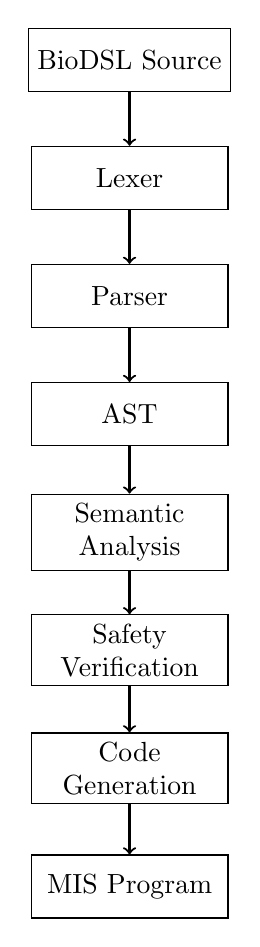
\begin{tikzpicture}[
    node distance=1.5cm,
    box/.style={rectangle, draw, minimum width=2.5cm, minimum height=0.8cm, align=center},
    arrow/.style={->, thick}
]
    \node[box] (source) {BioDSL Source};
    \node[box, below of=source] (lexer) {Lexer};
    \node[box, below of=lexer] (parser) {Parser};
    \node[box, below of=parser] (ast) {AST};
    \node[box, below of=ast] (semantic) {Semantic\\Analysis};
    \node[box, below of=semantic] (safety) {Safety\\Verification};
    \node[box, below of=safety] (codegen) {Code\\Generation};
    \node[box, below of=codegen] (mis) {MIS Program};

    \draw[arrow] (source) -- (lexer);
    \draw[arrow] (lexer) -- (parser);
    \draw[arrow] (parser) -- (ast);
    \draw[arrow] (ast) -- (semantic);
    \draw[arrow] (semantic) -- (safety);
    \draw[arrow] (safety) -- (codegen);
    \draw[arrow] (codegen) -- (mis);
\end{tikzpicture}
\caption{BioDSL compilation pipeline}
\end{figure}

\subsection{Lexical Analysis}

The lexer, implemented using the Logos tokenizer framework, recognizes BioDSL tokens including:

\begin{itemize}
    \item Keywords: \texttt{molecule}, \texttt{genetic\_circuit}, \texttt{protein}, \texttt{synthesize}
    \item Chemistry tokens: \texttt{benzene}, \texttt{pyran}, \texttt{hydroxyl}, \texttt{methyl}
    \item Stereochemistry: \texttt{R}, \texttt{S}, \texttt{E}, \texttt{Z}
    \item Robot commands: \texttt{robot\_swarm}, \texttt{NanoQuantumonas}, \texttt{atomic\_assembly}
    \item Units: \texttt{mg}, \texttt{ug}, \texttt{mol}, \texttt{mmol}
\end{itemize}

\subsection{Abstract Syntax Tree}

The parser generates an AST that preserves structural relationships:

\begin{lstlisting}[language=Rust,caption={Core AST structures}]
pub struct MoleculeDefinition {
    pub name: String,
    pub smiles: Option<String>,
    pub scaffold: Option<ScaffoldDefinition>,
    pub substituents: Vec<SubstituentDefinition>,
    pub stereocenters: Vec<StereocenterDefinition>,
    pub synthesis_method: Option<SynthesisMethod>,
    pub verification: Option<VerificationSpec>,
}

pub struct GeneticCircuitDefinition {
    pub name: String,
    pub promoters: Vec<PromoterDefinition>,
    pub genes: Vec<GeneDefinition>,
    pub interactions: Vec<Interaction>,
    pub inputs: Vec<CircuitInput>,
    pub outputs: Vec<CircuitOutput>,
    pub safety: Option<SafetyFeatures>,
}
\end{lstlisting}

\subsection{Molecular Instruction Set}

The compiler generates instructions in the Molecular Instruction Set (MIS), a low-level representation optimized for robot execution:

\begin{table}[H]
\centering
\begin{tabular}{lp{8cm}}
\toprule
\textbf{Instruction} & \textbf{Description} \\
\midrule
\texttt{PlaceAtom} & Position an atom at specified 3D coordinates with quantum precision \\
\texttt{FormBond} & Create a chemical bond between two positioned atoms \\
\texttt{LaserPulse} & Apply attosecond laser pulse for bond activation/breaking \\
\texttt{VerifyStructure} & Quantum tomography verification of molecular structure \\
\texttt{AssembleRing} & Construct aromatic or aliphatic ring system \\
\texttt{BuildMOF} & Construct metal-organic framework structure \\
\texttt{SynthesizeDNA} & Assemble DNA sequence from nucleotides \\
\texttt{AssistProteinFolding} & Guide protein folding with quantum coherence \\
\bottomrule
\end{tabular}
\caption{Core Molecular Instruction Set operations}
\end{table}

\section{Robot Swarm Integration}

BioDSL programs are executed by specialized quantum water robot swarms. Each robot type is optimized for specific operations:

\begin{table}[H]
\centering
\begin{tabular}{lp{7cm}}
\toprule
\textbf{Robot Type} & \textbf{Specialization} \\
\midrule
NanoQuantumonas & Atomic-precision atom placement and bond formation \\
QuantumJellyfish & Metal-organic framework (MOF) construction \\
TunnelingOctopus & Zeolitic imidazolate framework (ZIF) assembly \\
EntangledDolphin & Covalent organic framework (COF) building \\
CyberCetus & Protein folding assistance \\
SchoolingRobotichthys & Parallel distributed operations \\
\bottomrule
\end{tabular}
\caption{Quantum water robot types and their specializations}
\end{table}

The compiler automatically selects optimal robot types for each instruction based on the operation requirements.

\section{Biosafety Framework}

BioDSL implements comprehensive safety controls to prevent misuse while enabling legitimate research.

\subsection{Prohibited Molecules}

The safety controller maintains a list of absolutely prohibited molecules that cannot be synthesized under any circumstances:

\begin{itemize}
    \item Biological warfare agents (ricin, botulinum toxin)
    \item Chemical weapons (VX, sarin, novichok agents)
    \item Highly dangerous pathogens
\end{itemize}

\subsection{Controlled Substances}

Molecules classified as controlled substances require appropriate licensing:

\begin{lstlisting}[style=biodsl,caption={Controlled substance synthesis with licensing}]
synthesize THC {
    amount: 50mg
    purity: 99.5%
    license: "DEA-RESEARCH-2026-0001"
    purpose: "analytical_standard"
}
\end{lstlisting}

Quantity limits are enforced per-synthesis and per-day:

\begin{table}[H]
\centering
\begin{tabular}{lccc}
\toprule
\textbf{Substance} & \textbf{Schedule} & \textbf{Per Synthesis} & \textbf{Daily Limit} \\
\midrule
THC & I & 100mg & 500mg \\
CBD & -- & 10g & 100g \\
Psilocybin & I & 50mg & 200mg \\
Caffeine & -- & 100g & Unlimited \\
\bottomrule
\end{tabular}
\caption{Quantity limits for controlled substances}
\end{table}

\subsection{Genetic Circuit Safety}

All genetic circuits must include safety features:

\begin{enumerate}
    \item \textbf{Auxotrophy}: Metabolic dependency preventing environmental survival
    \item \textbf{Kill Switch}: Mechanisms for circuit termination (temperature-sensitive, toxin-antitoxin)
    \item \textbf{Generation Limits}: Maximum replication cycles
    \item \textbf{Containment Level}: BSL-1 through BSL-4 classification
\end{enumerate}

\section{Small Molecule Library}

BioDSL includes a pre-built library of common molecules with verified synthesis pathways:

\subsection{Cannabinoids}
\begin{itemize}
    \item $\Delta^9$-THC (Tetrahydrocannabinol)
    \item CBD (Cannabidiol)
    \item CBN (Cannabinol)
    \item CBG (Cannabigerol)
    \item $\Delta^8$-THC
    \item THCA (Tetrahydrocannabinolic acid)
\end{itemize}

\subsection{Terpenes}
\begin{itemize}
    \item Limonene (citrus)
    \item Myrcene (earthy)
    \item $\alpha$-Pinene (pine)
    \item Linalool (floral)
    \item $\beta$-Caryophyllene (spicy)
\end{itemize}

\subsection{Pharmaceuticals}
\begin{itemize}
    \item Aspirin (acetylsalicylic acid)
    \item Ibuprofen
    \item Melatonin
    \item Dopamine
    \item Caffeine
\end{itemize}

\section{Genetic Circuit Templates}

BioDSL provides verified templates for common synthetic biology constructs:

\subsection{Toggle Switch}

The Gardner-Collins toggle switch provides bistable gene expression controlled by two inducers.

\begin{equation}
\frac{d[u]}{dt} = \frac{\alpha_1}{1 + [v]^{\beta}} - [u]
\end{equation}
\begin{equation}
\frac{d[v]}{dt} = \frac{\alpha_2}{1 + [u]^{\gamma}} - [v]
\end{equation}

\subsection{Repressilator}

The Elowitz-Leibler repressilator provides oscillatory gene expression through a three-node repression cycle.

\subsection{AND Gate}

Logic gates enable complex biological computation:

\begin{lstlisting}[style=biodsl,caption={BioDSL AND gate implementation}]
genetic_circuit ANDGate {
    input A: arabinose_induced
    input B: IPTG_induced

    gene gfp {
        requires: [A, B]
        product: "GFP reporter"
    }

    output: fluorescence when (A AND B)
}
\end{lstlisting}

\section{On-Chain Verification}

BioDSL synthesis operations integrate with Q-NarwhalKnight's quantum consensus system for trustless verification.

\subsection{Synthesis Proofs}

Each synthesis operation generates a cryptographic proof:

\begin{enumerate}
    \item \textbf{Program Hash}: SHA3-256 hash of the compiled MIS program
    \item \textbf{Execution Trace}: Merkle root of instruction execution states
    \item \textbf{Verification Data}: Quantum tomography results
    \item \textbf{Safety Attestation}: Cryptographic proof of safety constraint satisfaction
\end{enumerate}

\subsection{DAG-Knight Integration}

Synthesis proofs are recorded in the Q-NarwhalKnight DAG structure:

\begin{lstlisting}[language=Rust,caption={Synthesis proof vertex}]
struct SynthesisProofVertex {
    program_hash: [u8; 32],
    molecule_id: String,
    execution_trace: MerkleRoot,
    verification_status: VerificationStatus,
    safety_attestation: SafetyProof,
    timestamp: u64,
    signatures: Vec<QuantumSignature>,
}
\end{lstlisting}

\section{Blockchain Smart Contract Integration}

BioDSL integrates with Q-NarwhalKnight's smart contract ecosystem to provide trustless licensing, verification, tokenized rights, and decentralized safety governance. This section describes the five core bio-smart contracts that enable on-chain biological programming compliance.

\subsection{BioLicense Contract}

The BioLicense contract manages DEA-compliant licensing for controlled substance synthesis:

\begin{lstlisting}[language=Rust,caption={BioLicense contract interface}]
pub struct BioLicense {
    pub license_id: [u8; 32],
    pub holder: Address,
    pub license_type: LicenseType,
    pub max_schedule: DEASchedule,
    pub daily_quantity_limit_mg: u64,
    pub authorized_molecules: Vec<[u8; 32]>,
    pub expiration_block: u64,
    pub authority_signature: [u8; 64],
}

pub enum DEASchedule {
    ScheduleI,    // Highest restriction
    ScheduleII,   // High abuse potential
    ScheduleIII,  // Moderate potential
    ScheduleIV,   // Low potential
    ScheduleV,    // Lowest potential
    ResearchOnly, // Academic/research use
    Unscheduled,  // No restrictions
}
\end{lstlisting}

The BioLicense contract provides:

\begin{itemize}
    \item \textbf{On-chain License Verification}: Real-time verification of DEA/FDA compliance before synthesis
    \item \textbf{Quantity Tracking}: Daily and per-synthesis quantity limits enforced on-chain
    \item \textbf{Molecule Authorization}: Cryptographic binding between licenses and specific molecules
    \item \textbf{Expiration Management}: Automatic license expiration at specified block heights
    \item \textbf{Authority Signatures}: Government authority signatures for license validity
\end{itemize}

\subsection{SynthesisProof Contract}

The SynthesisProof contract creates immutable, verifiable records of synthesis operations:

\begin{lstlisting}[language=Rust,caption={SynthesisProof contract interface}]
pub struct SynthesisProof {
    pub proof_id: [u8; 32],
    pub synthesis_id: [u8; 32],
    pub molecule_hash: [u8; 32],
    pub synthesizer: Address,
    pub license_id: [u8; 32],
    pub verification_method: VerificationMethod,
    pub quantum_signature: [u8; 64],
    pub timestamp: u64,
    pub block_height: u64,
}

pub enum VerificationMethod {
    QuantumTomography,     // Full quantum state verification
    SpectroscopicAnalysis, // NMR/MS/IR verification
    CrystallographicProof, // X-ray structure proof
    ComputationalMatch,    // Structure prediction match
    SwarmnessAttestation,  // Robot swarm consensus
}
\end{lstlisting}

Features include:

\begin{itemize}
    \item \textbf{Immutable Records}: Synthesis proofs cannot be modified after recording
    \item \textbf{Multi-Method Verification}: Support for quantum, spectroscopic, and computational verification
    \item \textbf{Chain of Custody}: Complete traceability from synthesis to final product
    \item \textbf{Dispute Resolution}: On-chain challenge mechanism for verification disputes
\end{itemize}

\subsection{BioToken Contract}

BioToken (BDSL) is an ERC20-compatible token for synthesis rights and governance:

\begin{lstlisting}[language=Rust,caption={BioToken staking tiers}]
pub struct BioTokenContract {
    pub total_supply: u128,
    pub staking_pools: HashMap<StakingTier, StakingPool>,
    pub synthesis_fee_rate: u64,   // Basis points
    pub oracle_reward_rate: u64,
}

pub enum StakingTier {
    Basic,       // 1,000 BDSL - Basic synthesis rights
    Researcher,  // 10,000 BDSL - Research privileges
    Laboratory,  // 100,000 BDSL - Lab-scale synthesis
    Industrial,  // 1,000,000 BDSL - Industrial capacity
    Oracle,      // 500,000 BDSL - Safety oracle voting
}
\end{lstlisting}

Token economics:

\begin{table}[H]
\centering
\begin{tabular}{lccc}
\toprule
\textbf{Staking Tier} & \textbf{Min Stake} & \textbf{Synthesis Limit} & \textbf{Oracle Weight} \\
\midrule
Basic & 1,000 BDSL & 10mg/day & -- \\
Researcher & 10,000 BDSL & 100mg/day & $1\times$ \\
Laboratory & 100,000 BDSL & 10g/day & $5\times$ \\
Industrial & 1,000,000 BDSL & 1kg/day & $20\times$ \\
Oracle & 500,000 BDSL & -- & $10\times$ \\
\bottomrule
\end{tabular}
\caption{BioToken staking tiers and privileges}
\end{table}

\subsection{BioSafety Oracle Contract}

The BioSafety Oracle provides decentralized safety classification through stake-weighted voting:

\begin{lstlisting}[language=Rust,caption={BioSafety Oracle interface}]
pub struct BioSafetyOracleContract {
    pub oracles: HashMap<Address, OracleInfo>,
    pub classifications: HashMap<[u8; 32], SafetyClassification>,
    pub pending_votes: HashMap<[u8; 32], Vec<SafetyVote>>,
    pub quorum_threshold: u64,    // Minimum votes required
    pub consensus_threshold: u64,  // % agreement needed
}

pub struct SafetyClassification {
    pub molecule_hash: [u8; 32],
    pub classification: SafetyLevel,
    pub dea_schedule: Option<DEASchedule>,
    pub special_restrictions: Vec<String>,
    pub consensus_weight: u64,
    pub last_updated_block: u64,
}

pub enum SafetyLevel {
    Safe,                    // Unrestricted synthesis
    RequiresLicense,         // DEA/FDA license needed
    ResearchOnly,            // Academic only
    Prohibited,              // Absolutely forbidden
    PendingClassification,   // Under review
}
\end{lstlisting}

Oracle governance features:

\begin{itemize}
    \item \textbf{Stake-Weighted Voting}: Higher stakes provide proportionally more voting power
    \item \textbf{Quorum Requirements}: Minimum participation threshold for valid classifications
    \item \textbf{Slashing Conditions}: Malicious or negligent oracles lose staked tokens
    \item \textbf{Appeal Process}: Disputed classifications can be challenged with bond
    \item \textbf{Regulatory Integration}: Authority override for legal compliance
\end{itemize}

\subsection{SynthesisMarketplace Contract}

The SynthesisMarketplace enables peer-to-peer synthesis services with escrow:

\begin{lstlisting}[language=Rust,caption={Marketplace contract structures}]
pub struct SynthesisListing {
    pub listing_id: [u8; 32],
    pub provider: Address,
    pub molecule_hash: [u8; 32],
    pub price_per_mg: u64,        // In BDSL tokens
    pub max_quantity_mg: u64,
    pub min_order_mg: u64,
    pub turnaround_blocks: u64,
    pub verification_method: VerificationMethod,
    pub provider_stake: u64,      // Quality bond
}

pub struct SynthesisOrder {
    pub order_id: [u8; 32],
    pub listing_id: [u8; 32],
    pub customer: Address,
    pub quantity_mg: u64,
    pub total_price: u64,
    pub escrow_amount: u64,
    pub status: OrderStatus,
    pub deadline_block: u64,
}

pub enum OrderStatus {
    Pending,     // Order placed, awaiting acceptance
    Accepted,    // Provider accepted, synthesis in progress
    Synthesized, // Synthesis complete, verification pending
    Verified,    // Proof verified, awaiting delivery
    Delivered,   // Product delivered, customer confirmation
    Completed,   // Payment released to provider
    Disputed,    // Under dispute resolution
    Cancelled,   // Order cancelled
}
\end{lstlisting}

Marketplace features:

\begin{itemize}
    \item \textbf{Escrow Protection}: Customer funds held in escrow until verified delivery
    \item \textbf{Quality Bonds}: Providers stake tokens as quality guarantee
    \item \textbf{Reputation System}: On-chain history of successful completions
    \item \textbf{Automated Verification}: Integration with SynthesisProof contract
    \item \textbf{Dispute Resolution}: Stake-backed arbitration for disagreements
\end{itemize}

\subsection{Cross-Contract Integration}

The bio-smart contracts form an integrated ecosystem:

\begin{figure}[H]
\centering
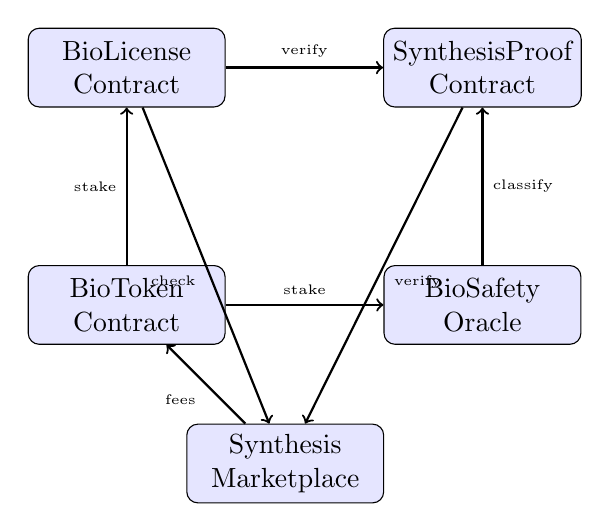
\begin{tikzpicture}[
    node distance=2cm,
    contract/.style={rectangle, draw, rounded corners, minimum width=2.5cm, minimum height=1cm, align=center, fill=blue!10},
    arrow/.style={->, thick}
]
    \node[contract] (license) {BioLicense\\Contract};
    \node[contract, right=of license] (proof) {SynthesisProof\\Contract};
    \node[contract, below=of license] (token) {BioToken\\Contract};
    \node[contract, below=of proof] (oracle) {BioSafety\\Oracle};
    \node[contract, below right=1cm and -0.5cm of token] (market) {Synthesis\\Marketplace};

    \draw[arrow] (license) -- node[above,font=\tiny] {verify} (proof);
    \draw[arrow] (token) -- node[left,font=\tiny] {stake} (license);
    \draw[arrow] (oracle) -- node[right,font=\tiny] {classify} (proof);
    \draw[arrow] (token) -- node[above,font=\tiny] {stake} (oracle);
    \draw[arrow] (market) -- node[below left,font=\tiny] {fees} (token);
    \draw[arrow] (license) -- node[below left,font=\tiny] {check} (market);
    \draw[arrow] (proof) -- node[below right,font=\tiny] {verify} (market);
\end{tikzpicture}
\caption{Bio-smart contract ecosystem integration}
\end{figure}

\subsubsection{Pre-Synthesis Workflow}

Before any synthesis operation, BioDSL performs on-chain verification:

\begin{enumerate}
    \item \textbf{License Check}: Verify synthesizer holds valid BioLicense
    \item \textbf{Safety Query}: Query BioSafety Oracle for molecule classification
    \item \textbf{Stake Verification}: Ensure adequate BioToken stake for synthesis tier
    \item \textbf{Quantity Validation}: Check daily limits haven't been exceeded
    \item \textbf{Authorization}: Generate cryptographic authorization for synthesis
\end{enumerate}

\begin{lstlisting}[language=Rust,caption={Pre-synthesis blockchain check}]
pub async fn pre_synthesis_check(
    molecule: &MoleculeDefinition,
    synthesizer: Address,
    quantity_mg: u64,
) -> Result<PreSynthesisApproval, BioContractError> {
    // 1. Check license validity
    let license = bio_license_contract
        .get_license(synthesizer)
        .await?
        .ok_or(BioContractError::NoValidLicense)?;

    // 2. Query safety oracle
    let classification = bio_safety_oracle
        .get_classification(molecule.hash())
        .await?;

    // 3. Verify authorization
    if classification.requires_schedule() > license.max_schedule {
        return Err(BioContractError::InsufficientLicense);
    }

    // 4. Check quantity limits
    if quantity_mg > license.daily_remaining_mg().await? {
        return Err(BioContractError::QuantityExceeded);
    }

    Ok(PreSynthesisApproval::new(license, classification))
}
\end{lstlisting}

\subsubsection{Post-Synthesis Recording}

After successful synthesis, proofs are recorded on-chain:

\begin{lstlisting}[language=Rust,caption={Post-synthesis proof recording}]
pub async fn record_synthesis_proof(
    molecule: &MoleculeDefinition,
    verification_data: &VerificationData,
    approval: &PreSynthesisApproval,
) -> Result<OnChainProof, BioContractError> {
    // Generate synthesis proof
    let proof = SynthesisProof {
        synthesis_id: generate_synthesis_id(),
        molecule_hash: molecule.hash(),
        verification_method: verification_data.method,
        quantum_signature: sign_with_quantum_key(verification_data),
        timestamp: current_timestamp(),
        block_height: current_block_height(),
    };

    // Record on-chain
    let proof_id = synthesis_proof_contract
        .record_proof(proof)
        .await?;

    // Update daily synthesis totals
    bio_license_contract
        .record_synthesis(approval.license_id, quantity_mg)
        .await?;

    Ok(OnChainProof { proof_id, ..proof })
}
\end{lstlisting}

\section{Performance Considerations}

\subsection{Compilation Time}

The BioDSL compiler is optimized for fast iteration:

\begin{table}[H]
\centering
\begin{tabular}{lc}
\toprule
\textbf{Operation} & \textbf{Time} \\
\midrule
Lexing (1000 tokens) & $<$ 1ms \\
Parsing (small molecule) & $<$ 5ms \\
Parsing (genetic circuit) & $<$ 20ms \\
Safety verification & $<$ 10ms \\
Code generation & $<$ 50ms \\
\bottomrule
\end{tabular}
\caption{Typical compilation times}
\end{table}

\subsection{Synthesis Estimation}

The compiler estimates synthesis time based on molecular complexity:

\begin{equation}
T_{synthesis} = N_{atoms} \cdot t_{placement} + N_{bonds} \cdot t_{formation} + T_{verification}
\end{equation}

Where:
\begin{itemize}
    \item $N_{atoms}$: Number of atoms in the molecule
    \item $t_{placement}$: Average time for quantum-precise atom placement ($\approx$ 100$\mu$s)
    \item $N_{bonds}$: Number of chemical bonds
    \item $t_{formation}$: Average bond formation time ($\approx$ 50$\mu$s)
    \item $T_{verification}$: Quantum tomography verification time ($\approx$ 10ms)
\end{itemize}

\section{Future Directions}

\subsection{Planned Enhancements}

\begin{enumerate}
    \item \textbf{Reaction Pathway Optimization}: AI-assisted synthesis route planning
    \item \textbf{Multi-Robot Coordination}: Advanced swarm algorithms for parallel synthesis
    \item \textbf{Live Cell Integration}: In-vivo synthesis capabilities
    \item \textbf{Protein Design}: De novo protein engineering support
    \item \textbf{Metabolic Engineering}: Full metabolic pathway construction
\end{enumerate}

\subsection{Research Collaborations}

BioDSL is designed for integration with:

\begin{itemize}
    \item Rosetta protein design suite
    \item AlphaFold structure prediction
    \item KEGG metabolic pathways database
    \item PDB structural biology database
\end{itemize}

\section{Conclusion}

BioDSL provides a powerful abstraction layer for programming quantum water robots to perform biological synthesis. By combining expressive language design, comprehensive safety controls, and integration with Q-NarwhalKnight's trustless consensus system, BioDSL enables a new paradigm of verifiable, precise, and safe biological manufacturing.

The open-source implementation is available at \url{https://github.com/q-narwhalknight/q-bio-dsl} under the Apache 2.0 license.

\section*{Acknowledgments}

This work was supported by the Q-NarwhalKnight Foundation and the Quantum Water Robotics Consortium.

\bibliographystyle{plain}
\begin{thebibliography}{9}

\bibitem{smiles}
Weininger, D. (1988). SMILES, a chemical language and information system. \textit{Journal of Chemical Information and Computer Sciences}, 28(1), 31-36.

\bibitem{toggle}
Gardner, T. S., Cantor, C. R., \& Collins, J. J. (2000). Construction of a genetic toggle switch in Escherichia coli. \textit{Nature}, 403(6767), 339-342.

\bibitem{repressilator}
Elowitz, M. B., \& Leibler, S. (2000). A synthetic oscillatory network of transcriptional regulators. \textit{Nature}, 403(6767), 335-338.

\bibitem{biobricks}
Knight, T. (2003). Idempotent vector design for standard assembly of BioBricks. \textit{MIT Artificial Intelligence Laboratory}.

\bibitem{waterrobots}
Q-NarwhalKnight Team (2025). Quantum Water Robots: Atomic-Precision Molecular Manufacturing. \textit{arXiv:2501.xxxxx}.

\bibitem{qnk}
Q-NarwhalKnight Foundation (2025). DAG-Knight: Quantum-Enhanced Byzantine Fault Tolerant Consensus. \textit{Q-NarwhalKnight Technical Report}.

\bibitem{biocontracts}
Q-NarwhalKnight Team (2026). Bio-Smart Contracts: Decentralized Compliance for Biological Manufacturing. \textit{Q-NarwhalKnight Technical Specification}.

\bibitem{defi}
Schär, F. (2021). Decentralized Finance: On Blockchain- and Smart Contract-Based Financial Markets. \textit{Federal Reserve Bank of St. Louis Review}, 103(2), 153-174.

\bibitem{oracles}
Breidenbach, L., et al. (2021). Chainlink 2.0: Next Steps in the Evolution of Decentralized Oracle Networks. \textit{Chainlink Labs Whitepaper}.

\end{thebibliography}

\end{document}
